\chapter{Literature Review}
\label{chap:lr}
\chaptermark{Second Chapter Heading}

\section{Frechet Inception Distance}
The Fréchet Inception Distance(FID) is the distance metric. Idea behind each distance metric is to extract features from two datasets of pictures and then calculate distance between two datasets. Resulting scalar will be result of the metric. Extracted features may also be called embeddings: it is a vector of low dimensionality with respect to the dimensionality of the image. For clarity, I have made a diagram of the FID metric as a example of distance metric.
\begin{figure}[hbt]
\centering
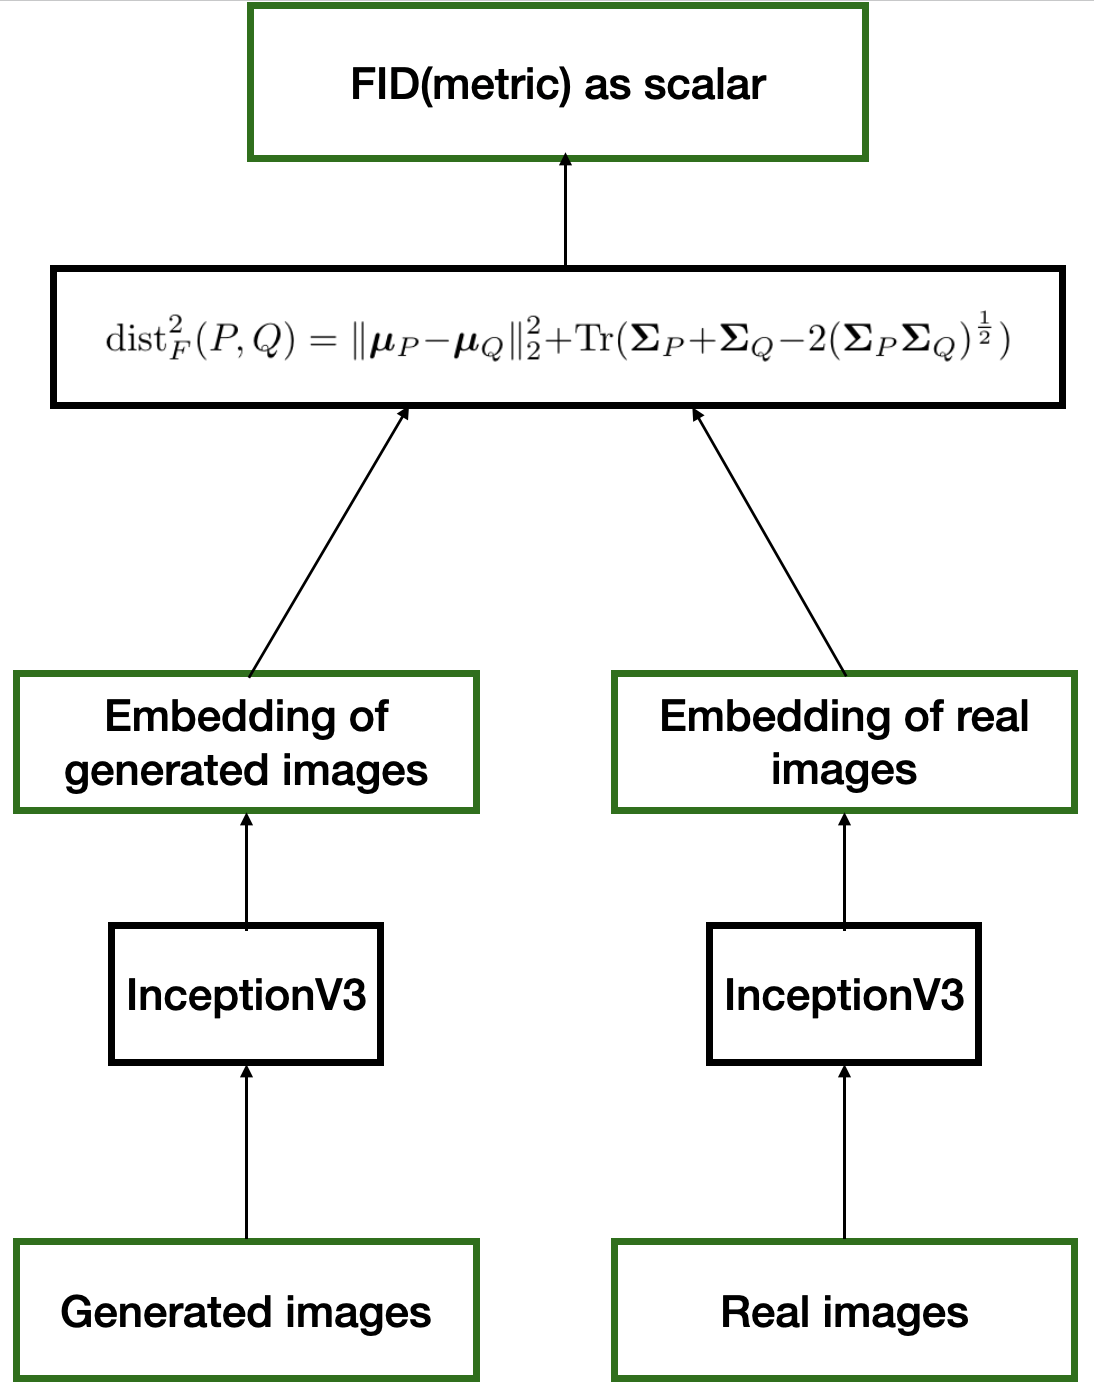
\includegraphics[width=10cm, height=12cm]{figs/fid_diagram.png}
\caption{The diagram of Fréchet Inception Distance(FID). Where $\mu_P$ , $\mu_Q$ are the means and $\Sigma_P$ , $\Sigma_Q$ are the covariances of the two multivariate normal distributions $P$ and $Q$}
\label{fig:FID_diagram}
\end{figure}
As show in the Figure~\ref{fig:FID_diagram}, fréchet inception distance (FID) metric uses the convolutional network InceptionV3 to compute image embeddings and fréchet distance for calculating distance between two datasets of embeddings.

The formula for calculating the Fréchet Distance taken from \cite{FD}:
\begin{equation}
dist^2_F(P,Q)=inf_{\gamma\in \Gamma(P,Q)}E_{(x,y)\gamma}\|x-y\|^2
\end{equation}
According to the authors of the \cite{KD_CLIP}: "$\Gamma(P, Q)$ is the set of all couplings of $P$ and $Q$. This is also equivalent to the Wasserstein-2 distance on $\mathbb{R}^d$. In general, obtaining a closed-form solution for the Fréchet distance is difficult". However, the authors of \cite{FD} showed that a closed-form solution exists for multivariate normal distributions in the form:
\begin{equation}
dist^2_F(P,Q)=\|\mu_P-\mu_Q\|_2^2+Tr(\Sigma_P+\Sigma_Q-2(\Sigma_P\Sigma_Q^{1/2})
\end{equation}
where $\mu_P$ , $\mu_Q$ are the means and $\Sigma_P$ , $\Sigma_Q$ are the covariances of the two multivariate normal distributions $P$ and $Q$. Formula (2.2) is valid only when both $P$ and $Q$ are multivariate normal distributions \cite{FD}.
\section{FID disadvantages}
The articles highlight several major disadvantages of FID. First, Sadeep highlights: "inception’s poor representation of the rich and varied content generated by modern text-to-image models" \cite[p.1]{KD_CLIP}. Analysis and improvement of existing offline metrics for evaluating the quality of diffusion models for text to image generation. Inception model \cite{InceptionV3} convolutional network that was trained for the classification task on the ImageNet dataset. Today, there are new network architectures that can replace inception network. Recent research papers  \cite{KD_CLIP}\cite{FD_DINOv2}\cite{FID_Med} have presented a critical analysis of the use of InceptionV3 in the FID metric. Evaluation results from previous studies \cite{KD_CLIP} revealed that FID may not reflect a person's actual view and may even increase with more steps in diffusion generative networks, when it is quite obvious that with more steps the image becomes better. Among the alternatives proposed, models such as DINOv2 \cite{DINOv2}(Distilled and Noisy Self-supervised learning framework) and CLIP \cite{CLIP}(Contrastive Language-Image Pretraining). The new feature extractors are expected to improve the metrics evaluation process, leading to more robust estimates of generative models.

Second, FID is biased as noted in \cite{unbiasedFID}. Due to FID is biased one model may receive a higher score than another just because one has a smaller bias term.

Third, fréchet distance require to calculate the $d \times d$ covariance matrix where $d$ is embedding's dimensionality. Since embeddings of images are high-dimensional, calculating of matrix is time consuming.

Fourth, use closed-form solution of fréchet distance justified if assumption about normality of two distributions is right. The claim that embeddings occur in a normal distribution has not been proved. This point will be revealed in feature chapters.

\section{CLIPScore model}
The CLIPScore is score metric. Idea behind each score metric is to extract features(embeddings) from prompt and generated image and calculate simmularity between two embeddings. Resulting scalar will be result of the metric.
\subsection{CLIP model}
For all score metrics which I found as feature extractors for prompts and generated images was used CLIP architecture \cite{CLIP} which showed in Figure~\ref{fig:CLIP}:
\begin{figure}[hbt]
\centering
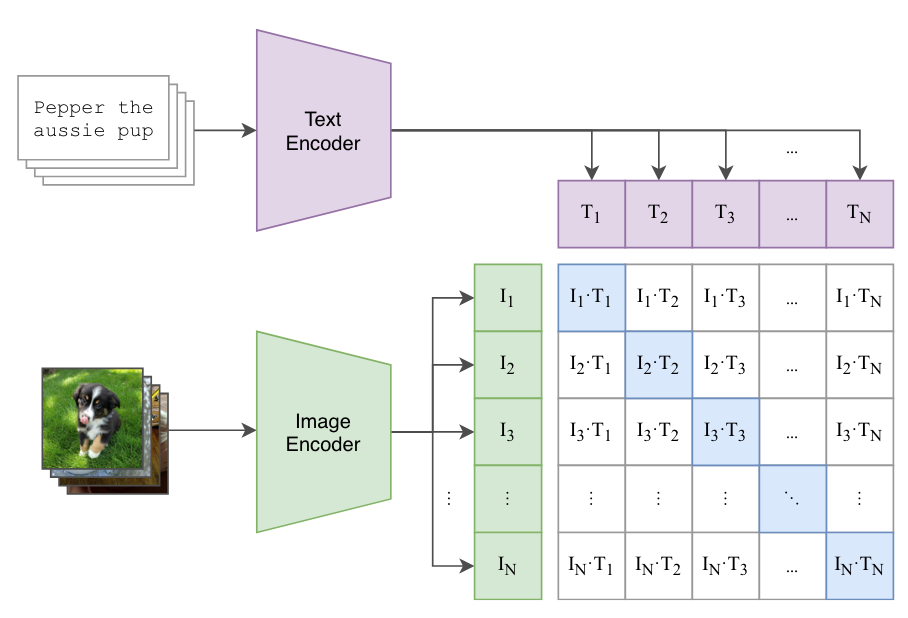
\includegraphics[width=12cm, height=8cm]{figs/clip.png}
\caption{Texts(prompts) and images encoded using Text Encoder and Image Encoder respectivly. Calculating cosine simularity for each pair of text and image from batch. CLIP architecture taken from \cite{CLIP}}
\label{fig:CLIP}
\end{figure}


The core idea behind CLIP is to align the image and text feature vectors in a high-dimensional space. Lets name the positive pair of image and text if we know that text associated to image and negative otherwise. Positive pairs of image and text should be close to each other in the feature space while negative pairs should be far apart. CLIP is trained on a large and diverse dataset collected from the internet, allowing it to learn from a broad range of visual styles, concepts, and natural language.


Once trained, CLIP can perform "zero-shot" learning, meaning it can correctly classify images into categories it has never seen during training, based only on textual descriptions of those categories. And also due to its training on a diverse internet-sourced dataset, CLIP generalizes well across different domains and types of images and descriptions.


To be clear I include pseudocode of CLIP training:
\begin{figure}[hbt]
\centering
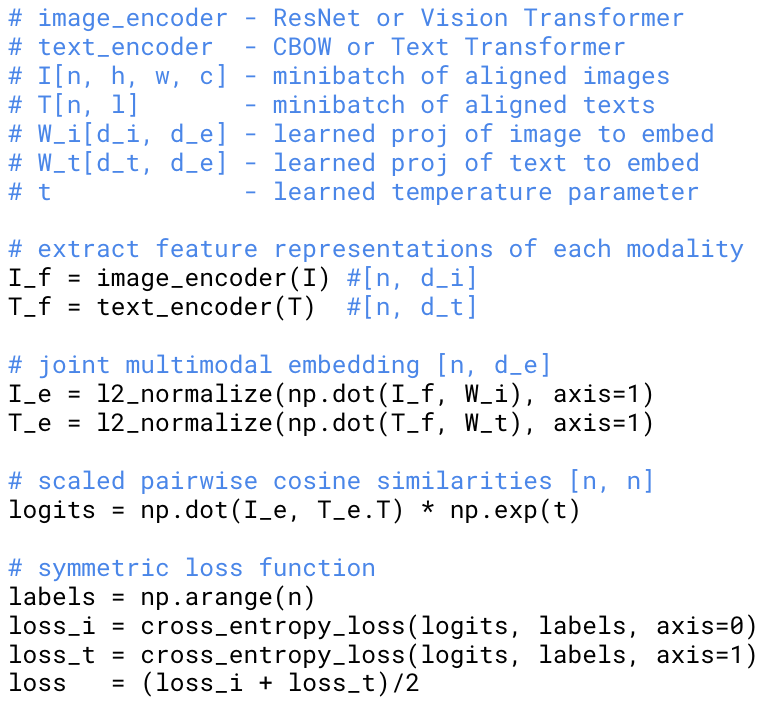
\includegraphics[width=12cm, height=10cm]{figs/clip_pseudocode.png}
\caption{Numpy-like pseudocode for the core of an implementation of CLIP. Taken from article\cite{CLIP}}
\label{fig:CLIP_pseudocode}
\end{figure}
\subsection{CLIP model for score metric}
CLIP  is trained so that cosine similarity of the image and text that describe image is close to 0 and close to 1 otherwise. I can use this property to determine the similarity of image and prompt. 

Hence, to calculate score of similarity of prompt and image using CLIP method I have to use text encoder and image encoder to encode prompt and image respectivly and then calculate cosine similarity between two embeddings.
\section{Other score models}
I found several articles \cite{DIffModels}\cite{PrecesionRecall}\cite{RarityScore} that describe metrics that do not refer to the types I have previously declared such as distance metric and score metric. These are such metrics as fidelity(precision) \cite{DIffModels}\cite{PrecesionRecall}, diversity(recall, coverage) \cite{DIffModels}\cite{PrecesionRecall}, memorization, mode collapse and rarity score \cite{RarityScore}.
\subsection{Precision and recall}
Precision and recall are well-known metrics in many areas of machine learning. Jiyeon Han proposed method for computing precision and recall metrics using k-nearest neighbor(KNN) method\cite{RarityScore}. Kynka¨anniemi et al. propose following method\cite{Precision_recall}: $X_r ~ P_r$ is real images distribution, $X_g ~ P_g$  is fake images distribution, then they embed them in feature space using pretrained model such as VGG16, InceptionV3 or CLIP. So they get set of real features(embedding) $\Phi_r$ and set of fake(generated) features $\Phi_g$. Then they proposed formula for manifold: 
\begin{equation}
\begin{split}
manifold_k(\Phi)=\bigcup_{\phi_i\in\Phi}B_k(\phi_i, \Phi),\\ B_k(\phi_i, \Phi)=\{\phi|d(\phi_i, \phi) <= NN_k(\phi_i,\Phi)\}
\end{split}
\end{equation}
Jiyeon highlights\cite{RarityScore}: "$NN_k(\phi_i, \Phi)$ represents the distance between $\phi_i$ and its k-th nearest neighbor in $\Phi$. $B_k(\phi_i, \Phi)$ is the k-NN sphere of $\phi_i$ with the radius of $NN_k(\phi_i, \Phi)$ defined as a set of all $\phi$ whose distance to $\phi_i$ is smaller than or equal to $NN_k(\phi_i, \Phi)$. For the distance metric d, we use L2 distance" \cite[p.2]{RarityScore}. Precision and recall formulas are declared as\cite{Precision_recall}:
\begin{equation}
precision(\Phi_r,\Phi_g)=\frac{1}{|\Phi_g|}\sum\limits_{\phi_j\in\Phi_g}I(\phi_j\in manifold_k(\Phi_r))
\end{equation}
\begin{equation}
recall(\Phi_r,\Phi_g)=\frac{1}{|\Phi_r|}\sum\limits_{\phi_i\in\Phi_r}I(\phi_i\in manifold_k(\Phi_g))
\end{equation}
where $I$ is indicator. Precision metric can be defined as fidelity and recall as diversity. So, in more common sense precision is the fraction of generated images that got in manifold of real images, recall is the fraction of real images that got in manifold of generated images. 
\subsection{Density and Coverage}
Precision and recall have several disadvantages: they are affected by outliers and are computationally inefficient. To overcome the disadvantages, density and coverage have been proposed\cite{Coverage_Density}.
\begin{equation}
density(\Phi_r,\Phi_g)=\frac{1}{k|\Phi_g|}\sum\limits_{\phi_j\in\Phi_g}\sum\limits_{\phi_i\in\Phi_r}I(\phi_j\in B_k(\phi_i,\Phi_r)
\end{equation}
\begin{equation}
coverate(\Phi_r,\Phi_g)=\frac{1}{|\Phi_r|}\sum\limits_{\phi_i\in\Phi_r}I(\exists\phi_i\in\Phi_g)
\end{equation}
Density may be more robust compared to precision due to if fake sample is in several k-NN spheres, then it more probably in manifold. 
And coverage may be more robust compared to recall. Jiyeon el al. highlights :"if a fake sample is sparsely located, the fake manifold can be exaggerated and the recall can be overestimated. As real manifold is known to have less outliers than the fake manifold, coverage can prevent such overestimation"\cite[p.3]{RarityScore}.
For a better understanding of metrics such as precision, recall, coverage, density, I provide a picture from the article\cite{Coverage_Density}:
\begin{figure}[hbt]
\centering
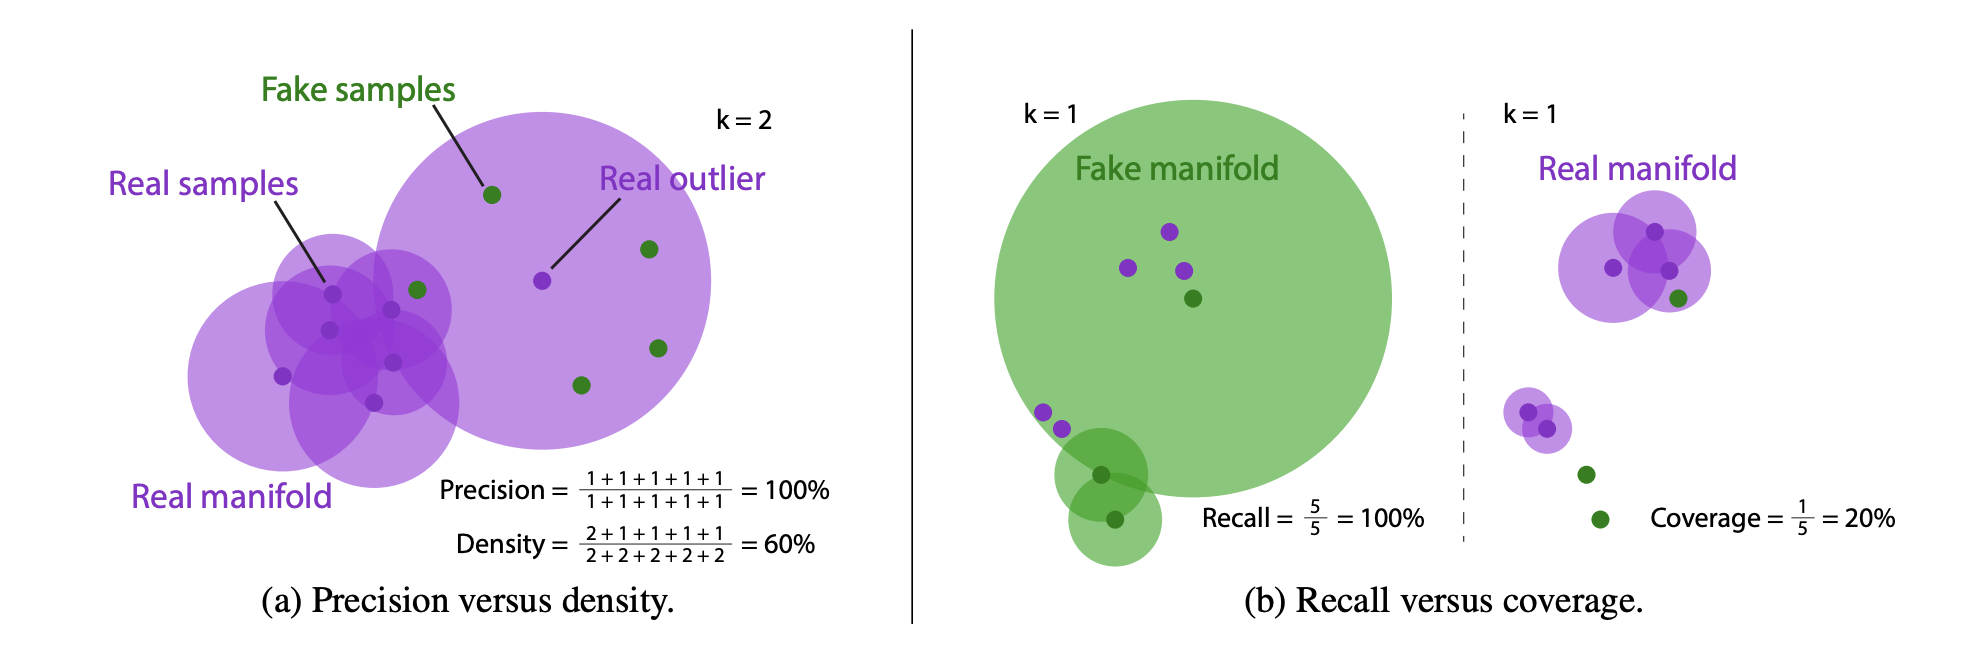
\includegraphics[width=15cm, height=7cm]{figs/precision_recall_coverage_density.png}
\caption{Two example scenarios for illustrating the advantage of density over precision and coverage over recall.
Note that for recall versus coverage figure, the real and fake samples are identical across left and right. Taken from article\cite{Coverage_Density}}
\label{fig:PrecisionRecallCoverageDensity}
\end{figure}
\subsection{Rarity score}
To calculalate 'rarity' of individual generation, Jiyeon el al. propose rariry score. They use KNN to represent manifold as Kynka¨anniemi et al.\cite{Precision_recall} make for precision and recall. Jiyeon writes: "We hypothesize that ordinary samples would be closer to each other whereas unique and rare samples would be sparsely located in the feature space"\cite[p.4]{RarityScore}. Formula of rarity score:
\begin{equation}
Rarity(\phi_g,\Phi_r)=\min_{r, s.t. \phi_g\in B_k(\phi_r,\Phi_r)}NN_k(\phi_r,\Phi_r)
\end{equation}
So, rarity score of a generated image is a radius of sphere of a
real images which contains the given generated image.

% \begin{longtable}{c|c}
% \caption[This is the title I want to appear in the List of Tables]{Simulation Parameters} \label{table:secsimulation_params} \\
% \hline
% A & B  \\
% \hline
% \endfirsthead
% \multicolumn{2}{@{}l}{} \\
% \hline
% A & B \\
% \hline
% \endhead
% \hline
%  \textbf{Parameter} & \textbf{Value}\\
%  \hline
%  Number of vehicles & $|\mathcal{V}|$\\
%  \hline
%  Number of RSUs & $|\mathcal{U}|$\\
%  \hline
%  RSU coverage radius & 150 m\\
%  \hline
%  V2V communication radius & 30 m\\
%  \hline
%  Smart vehicle antenna height & 1.5 m\\
%  \hline
%  RSU antenna height & 25 m\\
%  \hline
%  Smart vehicle maximum speed & $v_{max}$ m/s\\
%  \hline
%  Smart vehicle minimum speed & $v_{min}$ m/s\\
%  \hline
%  Common smart vehicle cache capacities & $[50, 100, 150, 200, 250]$ mb\\
%  \hline
%  Common RSU cache capacities & $[5000,1000,1500,2000,2500]$ mb\\
%  \hline
%  Common backhaul rates & $[75, 100, 150]$ mb/s\\
%  \hline
% \end{longtable}